%%%%%%%%%%%%%%%%%%%%%%% file template.tex %%%%%%%%%%%%%%%%%%%%%%%%%
%
% This is a general template file for the LaTeX package SVJour3
% for Springer journals.          Springer Heidelberg 2010/09/16
%
% Copy it to a new file with a new name and use it as the basis
% for your article. Delete % signs as needed.
%
% This template includes a few options for different layouts and
% content for various journals. Please consult a previous issue of
% your journal as needed.
%
%%%%%%%%%%%%%%%%%%%%%%%%%%%%%%%%%%%%%%%%%%%%%%%%%%%%%%%%%%%%%%%%%%%
%
% First comes an example EPS file -- just ignore it and
% proceed on the \documentclass line
% your LaTeX will extract the file if required
%\begin{filecontents*}{example.eps}
%!PS-Adobe-3.0 EPSF-3.0
%%BoundingBox: 19 19 221 221
%%CreationDate: Mon Sep 29 1997
%%Creator: programmed by hand (JK)
%%EndComments
\iffalse
gsave
newpath
  20 20 moveto
  20 220 lineto
  220 220 lineto
  220 20 lineto
closepath
2 setlinewidth
gsave
  .4 setgray fill
grestore
stroke
grestore
\end{filecontents*}
%
\RequirePackage{fix-cm}
%
%\documentclass{svjour3}                     % onecolumn (standard format)
%\documentclass[smallcondensed]{svjour3}     % onecolumn (ditto)
\documentclass[smallextended]{svjour3}       % onecolumn (second format)
%\documentclass[twocolumn]{svjour3}          % twocolumn
%
\smartqed  % flush right qed marks, e.g. at end of proof
%
\usepackage{graphicx}

\usepackage{times,amsmath}
%\documentstyle[times,art10]{article} % For LaTeX 2.09
\usepackage[numbers]{natbib}
\usepackage{graphicx}
\usepackage{subfigure}
\usepackage{amssymb}
\usepackage{amsbsy}
\usepackage{amsfonts}
\usepackage{algorithmic}
\usepackage{algorithm}
\usepackage{url} 
\usepackage{multirow}
\usepackage{color}


%
% \usepackage{mathptmx}      % use Times fonts if available on your TeX system
%
% insert here the call for the packages your document requires
%\usepackage{latexsym}
% etc.
%
% please place your own definitions here and don't use \def but
% \newcommand{}{}
%
% Insert the name of "your journal" with
% \journalname{myjournal}
%
\begin{document}
\fi
\iffalse
%\thanks{Grants or other notes
%about the article that should go on the front page should be
%placed here. General acknowledgments should be placed at the end of the article.}
%}
%\subtitle{Do you have a subtitle?\\ If so, write it here}

%\titlerunning{Short form of title}        % if too long for running head

\author{Gr\'egoire Mesnil \and
        Antoine Bordes \and
        Jason Weston \and
        Gal Chechik \and
        Yoshua Bengio
}

%\authorrunning{Short form of author list} % if too long for running head

\institute{Gr\'egoire Mesnil \at
            LISA, Universit\'e de Montr\'eal / LITIS Universit\'e de Rouen\\
            Montr\'eal, QC, Canada / Rouen, France\\
            \email{mesnilgr@iro.umontreal.ca}
          \and
          Antoine Bordes \at
            CNRS - Heudiasyc UMR 7253\\
            Universit\'e de Technologie de Compi\`egne, France\\
              \email{antoine.bordes@utc.fr}          
          \and
           Jason Weston\at
            Google,\\
            New York, NY, USA\\
            \email{jweston@google.com}
          \and
           Gal Chechick\at
            Google,\\
            Mountain View, CA, USA\\
            \email{gal@google.com}
          \and
           Yoshua Bengio \at
            LISA, Universit\'e de Montr\'eal\\
            Montr\'eal, QC, Canada\\
            \email{bengioy@iro.umontreal.ca}
}

\date{Received: date / Accepted: date}
% The correct dates will be entered by the editor
\fi


\chapter{Learning Semantic Representations of Objects and their Parts \label{chap:mlj}}

\def\reals{\mathbb{R}} % Real number symbol
\def\R{\mathbb{R}}
\def\LPhi{{L}}
\def\Y{{\cal Y}}
\def\Ysz{K}
\def\bard{d_{\bar{\o}}}
\def\Multiclass{{\sc Pamir}$^{IA}$~}
\def\argmax{\arg\max}

%\newcommand{\ybar}{{\bar{y}}}
%\newcommand{\Ybar}{n}
%\newcommand{\floor}[1]{\left \lfloor #1 \right \rfloor}
%\newcommand{\newL}{\tilde{L}}
%\newcommand{\newPhi}{\tilde{\Phi}}
%\newcommand{\proba}{\text{Pr}}


\def\blue#1{\emph{\textcolor{blue}{#1}}}
\def\black#1{\emph{\textcolor{black}{#1}}}
\def\red#1{{\bf\textcolor{red}{#1}}}
\def\nbfred#1{{\textcolor{red}{#1}}}

\newcommand{\floor}[1]{\left \lfloor #1 \right \rfloor}
\newcommand{\fix}{\marginpar{FIX}}
\newcommand{\new}{\marginpar{NEW}}
% \newcommand{\argmax}{\mar}
% \DeclareMathOperator*{\argmax}{arg\,max}

\iffalse
\maketitle

\begin{abstract}
    Recently, large scale image annotation datasets have been collected
  with millions of images and thousands of possible annotations.
  %
  Latent variable models, or embedding methods, that
  simultaneously learn semantic representations of object labels and
  image representations can provide tractable solutions on such tasks.
  %
  %% ANTOINE
  % We are interested in learning such semantic representations
  % both for the objects in an image, and the parts of those objects.
  %
  In this work, we are interested in jointly learning representations
  both for the objects in an image, and the parts of those objects, because 
  such deeper semantic representations could bring a leap forward in image 
  retrieval or browsing.
  %
  %Machine learning provides powerful tools for image retrieval.
  %
  Despite the size of these datasets, the amount of annotated
  data for objects and parts can be costly and may not be available.
  %
%  The performance of trained systems can be improved by increasing the amount 
%  and degree of annotation of training data, for instance 
%  by supplying images tagged with objects and
%  their parts.
  % 
%  Unfortunately, getting such precise annotation is costly and
%  unrealistic for the huge amount of readily available image data.
  % 
  In this paper, we propose to bypass this cost with a method able to
  learn to jointly label objects and parts without requiring 
  exhaustively labeled data.
  %
  We design a model architecture that can be 
  trained under a proxy supervision obtained by combining
  standard image annotation (from ImageNet) with semantic part-based
  within-label relations (from WordNet). 
  The model itself is designed to model both object image to object label
  similarities, and object label to object part label similarities 
  in a single joint system.
  %
  Experiments conducted on our combined data and a precisely
  annotated evaluation set demonstrate 
  the usefulness of our approach.
%\keywords{First keyword \and Second keyword \and More}
\end{abstract}
\fi

\section{Introduction}

% Gal: I simplified a bit 

Images and language are two complementary representations of
information, and learning to translate between the two is of great
interest. In one direction, the task of image annotation maps images
to words, and in the other direction, the task of image retrieval maps
words to images. Both the semantics of words and the semantics of
images play a key role in these two tasks, since an accurate mapping
is required to retrieve images and text that are semantically similar. At
the same time, there also exist complex semantic relations within each
modality that are important to model.  For example, between-objects
relations include the relation {\em X is a part of Y} and {\em X is an
instance of Y}, and similar relations exist in the semantics of text
terms. We wish to develop models that learn these types of semantic
relations across and within modalities simultaneously.

% Images and language are two complementary representations that it is
% of great interest to translate between.  Given one, we are often
% interested in the representation of the other, and the two possible
% mapping directions are known as the tasks of image retrieval and image
% annotation.  In either case, it is expected that the semantics of
% words and the semantics of images play a key role as we are interested
% in retrieving the semantically similar images and text in order to
% perform well at these tasks.
% Moreover, within only a single modality there are also complex
% semantic relationships that one could expect that it is also important
% to model.  For example between objects there are relations such as X
% is a part of Y or X is an instance of Y, similarly there are relations
% betwen the words as well.  We would like to develop models that learn
% all these type of semantic relationship simultaneously.

Automatic tools provided by machine learning
% have proven to be reliable and efficient, and 
can be designed to capture
the semantics described above.  However, in real applications both the
dictionary of possible words and the set of possible objects are large
and learning their semantics requires a large amount of training
data. Indeed, the performance of machine learning models highly
depends on the quality and size of their training data sets, so there
is a clear incentive to design methods able to handle the huge
resources now available.

In this work, we develop a machine learning method to learn the
semantics of words, objects and parts of objects that is efficient
enough to be trained on large scale datasets.  The method works by
learning a latent semantic representation for each possible word or
phrase, and each object and part. Each semantic concept has a
vectorial representation in a low dimensional embedding space, the
dimensions of which are learnt from data.
%Similarly, after representing images with a bag
%of visual terms, a vectorial representation for each term is also learnt.
In the low dimensional semantic embedding space we want to capture
similarities between words, objects and part of objects, e.g. so that
objects are related to their particular labels and parts in the space.
To do this we employ a loss function that optimizes the ranking of
words given an object, the loss function tries to get the correct
assignment near the top of the ranked list.

The task we consider is of automatically labeling images with the
objects in the scene as well as the parts of those objects.
Importantly, we are interested in object parts that can be viewed as
objects by themselves, like the flash bulb of a camera, or a wheel of a car.
This is different from the numerous unnamed parts of which every object
consists of. Identifying such ``parts that are objects'', can be
particularly useful in image retrieval and browsing, where a large amount of 
such precisely labeled data could potentially lead
to a compelling advance.
%
%
%
%The aim of proving performance relies on obtaining more
%detailed image annotations.  For example, instead of providing a
%single label for an image, one can list (label) all objects in a scene, possibly
%within given bounding boxes, as well as parts of these objects and
%their positions.
%
%
% ANTOINE
%
For example, this could allow to automatically extend image queries 
via semantic part-based bridges: when looking for images of a particular 
object (say a "car"), one could also be presented images of related object parts 
(such as "wheel" or "windshield" ). This would seamlessly enhance the browsing experience.
%
Unfortunately, although some limited datasets with this type of
labeling are available \citep{Yao:2007, labelme}, collecting such
deeply annotated data is costly and time consuming,
%
Moreover, although some image annotation tasks can benefit from
collecting indirect data, like the case of users clicking on images in
search engines or accompanying text surrounding images, there are not
any large scale applications that provide such evidence for object
parts in images that we are aware of.


%% 
In this work we hence also propose a training method to tackle this problem of labeling objects
and their parts in images without requiring any precisely labeled data.
%%
Our approach relies on a proxy supervision which bypasses the problem
of precise annotation by using part-based semantic information among labels.
%
Our model is composed of two ranking components: one for ranking
labels according to an image and one for ranking labels according to
another label.
%
The first component can be seen as a standard image annotation model
whereas the second one learns to give high ranks to pairs of
labels for which one is the part of the other.
%
The two components are trained jointly using combined data built from two sources (ImageNet and WordNet).

This paper builds upon previous work published by \citep{image-wsabie}.
%
However, the previous work has only focused on the standard image annotation setting, whereas 
the present version proposes jointly learning 
object and part representations.
% 
Hence, many new elements are provided including the word, object and part joint model, its training scheme, the proxy 
supervision setting, the ImageNet+WordNet dataset and all experimental results on it and on the LHI data set~\citep{Yao:2007}.

The paper is organized as follows. 
Section~\ref{sec:joint-word-object} describes learning joint latent semantic models for words and objects.
Section~\ref{sec:jmodels} presents our full image annotation model for learning 
latent semantic models over words, objects and their parts.
Section~\ref{sec:training} then describes how to train both types of model.
In particular, the form of the loss for supervised learning is first described,
and then we introduce
our proxy supervision setup for training objects and their parts when supervision is limited,
 and describe our corresponding custom data set.
Section~\ref{sec:rwork} describes related work on image annotation and
part-based approaches. An empirical evaluation  on our custom test set and on precisely labeled images from
the LHI data set is given in Section~\ref{sec:exp}.
Finally, Section~\ref{conclusion} concludes.

\section{Latent Semantic Word and Object Models}\label{sec:joint-word-object} \label{jwie}

Before we describe the model that learns the semantics of words,
objects and their parts we start with a simpler model of representing
only words and objects, previously described in \citep{image-wsabie}.
In this case, a large amount of supervised data can be obtained, and
we hence detail a supervised training criterion for learning the
appropriate ranking function. We will explain below how this setup is
extended to learning about objects and their parts.

The following model learns a single latent semantic feature representation 
where both objects in images and word annotations  are represented.
The mapping functions for the two views are different, but are learnt jointly
to optimize the supervised loss of interest for our final task (here, we concentrate on the task 
of annotating images). The method is described pictorially in Figure~\ref{fig:wsabie}.


\subsubsection*{Notation summary}

\begin{itemize}

\item ${\cal L}$ is a set depicted by the $K$ words of the
dictionary corresponding to the image annotations.

\item ${\cal I}$ is the raw pixel space of images (no constraints on the size
of the images).

\item $\Phi_{\cal I} : {\cal I}\rightarrow {\mathbb R}^{N}$ maps an image to
its sparse representation.

\item $\Phi_{\cal L} : {\cal L}\rightarrow {\mathbb N}$ maps an annotation to its
index in the dictionary.

\item $E_{\cal I} : {\cal I} \rightarrow {\mathbb R}^{D}$ {\it embeds} an
image to the semantic space.

\item $E_{\cal L} : {\cal L} \rightarrow {\mathbb R}^{D}$ {\it embeds} an
annotation to the same semantic space. In some cases, the semantic space for
annotations is different than the images semantic space (see
Section~\ref{sec:ops} about Unshared models).

\item $f_I : {\cal I} \times {\cal L} \rightarrow {\mathbb R}$ returns a score
defining the similarity between an annotation and an image.

\end{itemize}



Given an image $I_o$ containing an object we wish to learn a function 
$E_{\cal I} : {\cal I} \rightarrow {\mathbb R}^{D}$ that {\em embeds} the inferred
object $I_o$ into a low-dimensional semantic space (where $D$ is typically
50-100 dimensions and $E_{\cal I}(I_o)$ is the representation of $I_o$ in the
semantic space).  Simultaneously, given an annotation of an object $L_o$, we
wish to also learn a function $E_{\cal L} : {\cal L}  \rightarrow {\mathbb
R}^{D}$ that represents the annotation in the same semantic space.  Then, our
overall model takes the form: 

\[ f_I(I_o, L_o) = S( E_{\cal I}(I_o), E_{\cal L}(L_o)), \] 

where $S : {\mathbb R}^{D}\times {\mathbb R}^{D} \rightarrow
{\mathbb R}$ is a measure of similarity in the semantic embedding space {\it
e.g.} a dot product $S(x,y)=x^\top y$.

For the feature representation of images, we first employ a fixed 
mapping $\Phi_{\cal I}(\cdot)$ that transforms the pixel representation
 into an $N$-dimensional vector which in this paper is a high-dimensional 
and sparse feature representation, as is also 
commonly performed in other works. % \citep{grangier:2008:tpami,wsabie}.
Then, we transform this intermediate representation to the $D$-dimensional semantic space, via
a linear map using a  $D \times N$ matrix $V$ of parameters:

\[ E_{\cal I}(I_o)  = V \Phi_{\cal I}(I_o).\]

In our model there is a dictionary with $K$ possible labels that can be embedded
using $E_{\cal L}(\cdot)$.  Following other works dealing with embedding
representations for text \citep{Bengio-scholarpedia-2007,wsabie} for each label
we learn a $D$ dimensional vector that will represent the label, resulting in a
$D \times K$ dimensional matrix $W$ of parameters to learn for the $K$ labels:

\[ E_{\cal L}(L_o) = W_{\Phi_{\cal L}(L_o)}, \]

where $\Phi_{\cal L}(\cdot)$ maps from the particular label to its index in the
dictionary, and thus retrieves the relevant column of a $D \times K$ matrix
$W$. (Note that a
standard matrix product with a one-hot vector would perform the same operation.)

Finally, for $S$ we choose the dot product similarity in the semantic space, resulting in the final model:

\[ f_I(I_o, L_o) = (V \Phi_{\cal I}(I_o))^\top W_{\Phi_{\cal L}(L_o)},\]
  
Our goal is to rank the candidate annotations of a given image such
that the highest ranked annotations describe best the semantic content of
the image.  We will describe the training procedure in
Section~\ref{sec:training}.  

\begin{figure*}[t!]
  \begin{center}
    \resizebox{0.7\textwidth}{!}{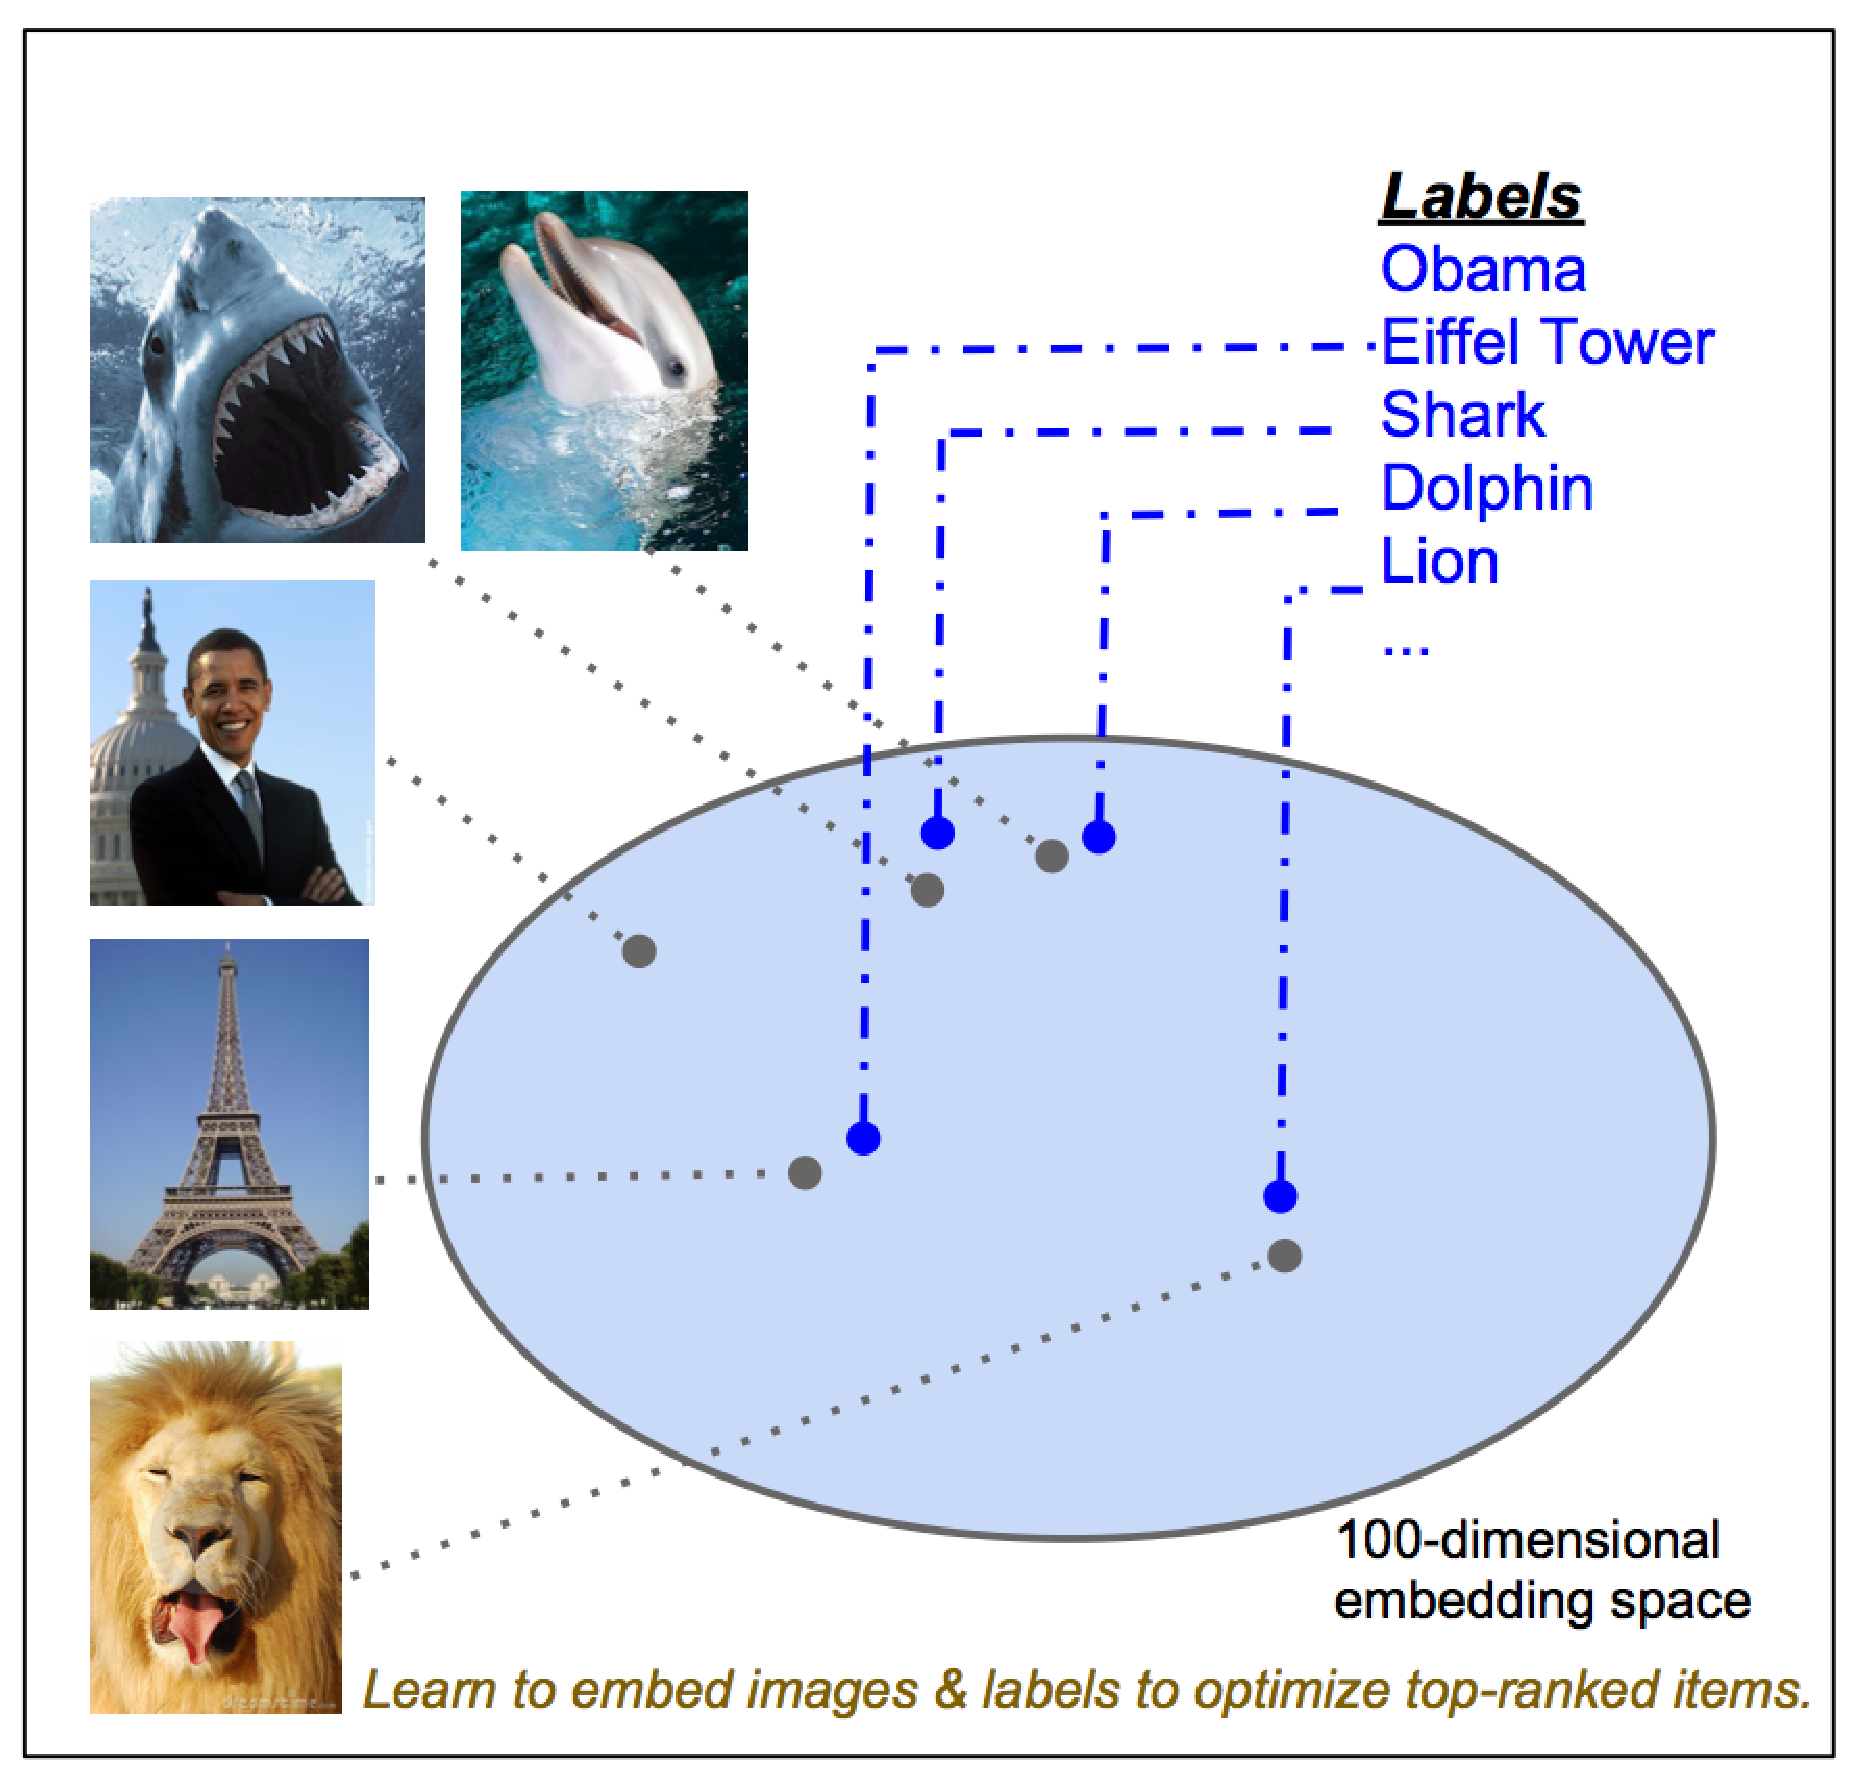
\includegraphics{article5/images/blah3.eps} }
    \caption[Latent Semantic Word and Object Models]{{\bf Learning Latent Semantic Word and Object Models.}}
    \label{fig:wsabie}
    \end{center}
\end{figure*}



\section{Latent Semantic Word, Object and Part Models}\label{sec:jmodels}
 

We want our model to simultaneously learn about objects being parts of scenes 
(a mapping from images to object labels) and about parts of objects
belonging to the objects (and again, the labels of those parts).
We hence now describe the generalization of the word, object model 
from the previous section to this case. 
%so that it also models
%parts (i.e., relations between objects in the image).

\subsubsection*{Notation summary}

\begin{itemize}

\item $f_L : {\cal L} \times {\cal L} \rightarrow {\mathbb R}$ returns a score
defining the similarity between an object annotation and a part annotation.

\item $f_q : {\cal I} \times {\cal L} \times {\cal I} \times {\cal L}
\rightarrow {\mathbb R}$ returns a score given a quadruplet of images and
annotations of a part and an object.

\item $f_I^U : {\cal I} \times {\cal L} \rightarrow {\mathbb R}$ differs from
$f_I$ since it has its own set of parameters and these parameters correspond
to the annotation embeddings that are not shared between the score functions $f_I^U$
and $f_L$. In this case, the annotations semantic space is different than the
images semantic space.

\end{itemize}


Our full model takes the form:

\[ f_q(I_o,L_o,I_p,L_p) = f_I(I_o,L_o) + f_I(I_p,L_p) + f_L(L_o,L_p) \]

where $I_o$ is the image in which an object of
interest is located, $I_p$ is the image in which an object part of interest is
located, $L_o$ is the label of the object and $L_p$ is the label of the part.
The function $f_q(I_o,L_o,I_p,L_p)$ which scores a given quadruplet of two
images and two labels is decomposed into three functions.  The function
$f_I(I_o,L_o)$ scores a given object label with the image of an object, and
$f_I(I_p,L_p)$ does the same for a part label with the image of a part.  The
last function $f_L$ scores the match between an object label and a part label.
(Note, we do not have a direct $f_{II}(I_o,I_p)$ term in our model to capture
image-image relationships directly although that is also possible.)
%Future work should investigate a $f_I(I_o,I_p)$ term to help better model
%images of parts that are actually inside the object image.



This model can be used in several setups.  Given the image of an object $I_o$
and a subregion of that image denoted with $I_p$, with no other prior
knowledge, we can label the object in $I_o$ and the part in $I_p$ with:

\[ \argmax_{L'_o,L'_p}  f_q(I_o,L'_o,I_p,L'_p).\]

If the object label  is already known and we are just looking for the names of
the parts we could fix $L_o$ as well:

\[ \argmax_{L'_p}  f_q(I_o,L_o,I_p,L'_p).\]

Finally, if we are only interested in labeling objects (and not their parts) we can use:

\[ \argmax_{L'_o}  f_I(I_o,L'_o).\]

The experiments below evaluate these different setups.  It now remains
to define the particular makeup of the functions $f_I$ and $f_L$.

As before, we assume that we are given a dictionary of $K$ possible
labels but now these labels are for both objects and parts, all in the
same dictionary. For example, a house has a door, and in turn, the
door has a handle, and so on.  Again, for each label we will learn a
$D$ dimensional vector that will represent it in the semantic space,
resulting in a $D \times K$ dimensional matrix $W$ of parameters to
learn for the $K$ labels.  The similarity between two labels is then
defined with:

\[ f_L(L_o, L_p) = W_{\Phi_{\cal L}(L_o)}^\top W_{\Phi_{\cal L}(L_p)},\]
%W_{L_o}^\top W_{L_p},\]

where $W_i$ indexes the $i^{th}$ column (label) of $W$. 

%We also constrain the norm of our parameters:
%\[
%  ||W_i|| \leq 1.
%\]

In the function $f_I$ we deal with images of parts and objects.
To measure similarity between an image and a label, we then have to transform them into 
the same space. This is again achieved with a fixed mapping $\Phi_{\cal I}(\cdot)$
and another $D \times N$ matrix $V$ of parameters:

\[ f_I(I, L) =  (V \Phi_{\cal I}(I) )^\top W_{\Phi_{\cal L}(L)},\]
%W_{L}.\]

%Here, we forced the functions $f_O$ and $f_P$ to be the same (shared parameters).

Note also that the label embeddings $W$ are also shared between all functions
$f_L$ and $f_I$.  In our experiments we also consider a ``non-sharing'' setting
where we decouple some of these parameters, so we instead consider:

\[ f_I^U(I, L)  =  (V \Phi_{\cal I}(I) )^\top U_{\Phi_{\cal L}(L)}, \]
%U_{L}.   \]

where $U$ is now a different set of parameters to $W$.

% Linear Embeddings models\citep{Weston:2010}

% 2 models: NNimage-word and NNword-word with shared weights for the word matrix

%** Evaluation settings: we use 3 setups:
%  1. standard: given an image, rank the label (only uses NNiw), this measure is used to show that our models performs well on a basic task.
%  2. 1 label: given a pair of images and a label, rank the remaining element of the triplet
%  3. pair: given a pair of images, rank the pairs of correct labels. We do not rank among all possible pairs (~1M!) but instead among 2k pairs, the 800 appearing in training and 1200 others randomly chosen.


%Some precisions:
%** f_O and  f_P share their weights (this is the same network actually)
%** for f_L and f_O/f_P, we have 2 settings whether they share the weights of the label embeddings matrix 
% or not (we termed them shared of unshared settings -- shared seems to work best but we wait final 
% results to be sure).

%Let me repeat that: f_O/f_P is exactly our WSABIE and f_L is the AAAI model without operator (you move closer  embeddings of labels linked by a part_of relation. Similarity measure between embeddings is the dot-product.



%thanks!

% ** Models: we are currently training 2 models. Both are composed of a NN scoring a pair 
% of words (denoted NNww) and a NN scoring a pair image-word (NNiw). Words and images encoded 
% via embeddings of size 50, the dot product between embeddings is used as similarity measure. 
%  The difference between our 2 model variants is that one shares the embeddings of the words 
% between NNww and NNiw (NNshared) and the other don't (NNunshared). We expect NNshared to outperform NNunshared.


\section{Training Our Models} \label{sec:training}

The two following sections (\ref{warp}, \ref{olmodel}) are taken from
previous work~\citep{image-wsabie} and describe the original object-label
setting and the WARP loss method. Afterwards, the object-parts model is built
upon that and described in detail in Section~\ref{sec:psup}. 

\subsection{Ranking Loss Function} \label{warp}
\newcommand{\ybar}{{\bar{y}}}
\newcommand{\Ybar}{n}
%\newcommand{\floor}[1]{\left \lfloor #1 \right \rfloor}
\newcommand{\newL}{\tilde{L}}
\newcommand{\newPhi}{\tilde{\Phi}}
\newcommand{\proba}{\text{Pr}}
We first consider the task of ranking labels $i \in {\cal Y}$ given  an image $x$,
i.e. the image annotation problem.
In our setting labeled pairs $(x,y)$ will be provided for training where
only a single annotation $y_i \in {\cal Y}$ is labeled correct\footnote{However, the methods described in this paper could be generalized to the multi-label case, naively by averaging the loss over all positive labels.}.
Let $f(x) \in \R^K$ be a vector function  providing a
score for each of the labels, where $f_i(x)$ is
the value for label $i$.

A classical loss function for learning to rank is to maximize AUC by minimizing:
\[
 err_{AUC}(f(x), y)  = \sum_x \sum_y \sum_{\ybar \neq y} \max(0,1+ f_{\ybar}(x) - f_y(x)),
\]
see, e.g.  \citep{herbrich2000large}.
This tries to make the positive label $y$ ranked above negative labels $\bar{y}$, because it sums
over all negative labels it optimizes the mean rank. It also enforces a margin of 1 as in margin-based 
methods like  SVMs \citep{svm}.
To make training of such a loss function scalable to large datasets 
with our model, one can optimize this loss using
 stochastic gradient descent (SGD):
sample triplets $(x, y, \bar{y})$ to make a gradient step on the hinge loss.

However, there is an issue with the loss above that, because all pairwise errors are the same 
(because it optimizes the mean rank), it may 
not be the best loss function for getting the correct label at the top of the ranked list (e.g. within the
top $k$). To give a simple example, 
suppose we are given only two functions to choose from, during our learning step we wish to  
pick the best one of the two.
Given two training images, if function 1 ranks their true labels at
position 1 and position 100 respectively, and function 2 ranks both at
position 50, then the AUC loss function prefers 
these functions equally as they both have 100 ``constraint violations'', 
assuming the margin is the same.
However, function 1 gives a superior precision at 1, because at least it gets one of the two examples correct.

To fix this problem, a class of ranking error functions was recently 
defined in~\citep{usunier:icml2009} as:
\begin{equation} \label{err-eq-orig}
err(f(x),y)  =  \LPhi(rank_y(f(x)))
\end{equation}
where $rank_y(f(x))$ is the rank of the true label $y$ given by $f(x)$:
\begin{equation*}
rank_y(f(x)) =  \sum_{i \neq y}  I( f_i(x) \geq f_y(x) )
\end{equation*}
where $I$ is the indicator function, 
and $\LPhi(\cdot)$ transforms this rank into a loss:
\begin{equation}
\label{def:lphi}
\LPhi(k)  =  \sum_{j=1}^k \alpha_j, \text{~with~} \alpha_1 \geq
\alpha_2\geq \dots \geq 0.
\end{equation}
This class of functions allows one to define different choices of $\LPhi(\cdot)$
with different minimizers. Minimizing $\LPhi$ with
$\alpha_j=\frac{1}{K-1}$ would optimize the mean rank, $\alpha_1=1$
and $\alpha_{j>1}=0$ the proportion of top-ranked correct
labels, and larger values of $\alpha$ in the first few positions optimize
the top $k$ in the ranked list, which is of interest for optimizing
precision at $k$. 
Now, given our example of two functions from before
where function 1 ranks their true labels at
position 1 and position 100 respectively, and function 2 ranks both at
position 50, then a choice of $\alpha_j=\frac{1}{K-1}$ prefers
these functions equally (just like AUC), whereas a choice of $\alpha_j=1/j$ prefers
the first function, which gives superior precision at 1.  

To optimize ~(\ref{err-eq-orig}) for large scale data one can also use stochastic gradient descent
by making updates of the parameters $\beta$ over randomly sampled examples and negative labels 
of the form:
\begin{equation}
\label{eq:sgdstep}
\beta_{t+1} = \beta_t - \gamma_t \frac{\partial \overline{err}(f(x),y,\bar{y})}{\partial \beta_t}.
\end{equation}
where $\gamma_t$ is the learning rate and
\[
\overline{err}(f(x),y,\bar{y}) = \LPhi(rank_y(f(x))) \max(1 - f_{\bar{y}}(x) + f_y(x), 0).
\]
Note the difference to the AUC optimization is just that 
the weighting of the update is now dependent on the
(current) rank of $y$.


\if 0
\subsubsection{Online Learning to Rank}
%
%We can rewrite the loss (\ref{err-eq-orig}) as:
The loss \eqref{err-eq-orig} is equal to:
\begin{equation*} 
%\label{err-eq}
err(f(x),y) =  \sum_{i \neq y}  \LPhi\left(rank_y(f(x))\right) \\  \frac{I( f_i(x) \geq f_y(x) )}{rank_y(f(x))}
\end{equation*}
with the convention $0/0=0$ when the correct label $y$ is
top-ranked. Using the hinge loss instead of the indicator function to
add a margin and make the loss continuous, $err$ can be approximated
by:
\begin{equation}
\label{err-eq}
\overline{err}(f(x),y) =  \sum_{i \neq y}  \LPhi\left(rank^1_y(f(x))\right) \\  \frac{\left|1- f_y(x) + f_i(x) \right|_+}{rank^1_y(f(x))}
\end{equation}
where $|t|_+$ is the positive part of $t$ and $rank^1_y(f(x))$ is the
margin-penalized rank of $y$:
\begin{equation} \label{eq-rank1}
rank^1_y(f(x)) = \sum_{i\neq y} I( 1+f_i(x) > f_y(x) ).
\end{equation}
The overall risk we want to minimize is then:
%are interested in minimizing can then be defined as:
\begin{equation} 
\label{risk}
Risk(f) = \int  \overline{err}(f(x),y)   dP(x,y).
\end{equation}
An unbiased estimator of this risk can be obtained by stochastically sampling in the following way:
\begin{enumerate}
\item Sample a pair $(x,y)$ according to $P(x,y)$;
\item For the chosen $(x,y)$ sample a violating label $\ybar$ such
  that $1+f_\ybar(x)>f_y(x)$.
% and  $\ybar \neq y$.
\end{enumerate}
This chosen triplet $(x,y,\ybar)$ has contribution:
\begin{equation}
\label{eq-err}
\overline{err}_{\ybar}(f(x),y,\ybar) = \LPhi(rank^1_y(f(x))) \left |1 - f_y(x)+ f_\ybar(x)\right|_+
\end{equation}
to the total risk, i.e. taking the expectation of these contributions
approximates (\ref{risk}) because we have  probability 
$1/rank^1_{y}(f(x))$ of drawing $\ybar$ in step (2) (or a contribution of 0 if 
$rank^1_{y}(f(x))=0$) which accounts for
the denominator of (\ref{err-eq}).

This suggests for learning we can thus perform the following stochastic update procedure~\citep{robbins_monro:1951} over the parameters $\beta$
 that define a family of possible functions $f \in {\cal F}$:
\begin{equation}
\label{eq:sgdstep}
\beta_{t+1} = \beta_t - \gamma_t \frac{\partial \overline{err}(f(x),y,\bar{y})}{\partial \beta_t}.
\end{equation}
where $\gamma_t$ is the learning rate.
% where
% \[
% \overline{err}(f(x),y,\bar{y}) = \LPhi(rank_y(f(x))) | 1 - f_i(x) + f_y(x) |_+
% \]
% and $|a|_+ = a$ if $a > 0$ and 0 otherwise. The use of the hinge loss instead
% of $I(\cdot)$ makes the loss differentiable and adds a margin.
\fi 

To perform this SGD step we still have the problem that computing  $rank^1_y(f(x))$  is quite inefficient:
to know the rank of $f_y(x)$ we have to compute the values $f_i(x)$ for  $i=1,\dots,K$.
However, there is a sampling trick that can solve this problem making it much more efficient:
the idea is that we can sample labels $i$ uniformly with replacement until we find a violating label. 
If there are $k=rank^1_y(f(x))$ violating labels, the random
variable $N_k$ which counts the number of trials in our sampling step
follows a geometric distribution of parameter $\frac{k}{K-1}$
(i.e. $\proba(N_k > q)\! =\!  (1-\frac{k}{K-1})^q$). Thus
$k=\frac{K-1}{E[N_k]}$. This suggests that the value of $rank^1_y(f(x))$
 may be approximated by:
$$rank^1_y(f(x)) \approx \floor{\frac{K-1}{N}}$$
where $\floor{.}$ is the floor function and $N$ the number of trials
in the sampling step.
This method is called the Weighted Approximate Ranked Pairwise (WARP) loss.

\subsection{Training Object and Label Models}
\label{olmodel}

Solving the image annotation problem with the semantic embedding model with objects and labels
hence consists of the
 joint word-image embedding model of Section \ref{jwie} trained with the WARP loss of Section \ref{warp}.
This method is called {\sc Wsabie} in \citep{image-wsabie}.
% and the pseudo code for the method is given in Algorithm~\ref{alg:wsabie}
The mapping matrices $V$ and $W$ are initialized at random
with mean 0, standard deviation $\frac{1}{\sqrt{d}}$, which is a common choice. 
%e.g. as implemented in the Torch Machine Learning
%library\footnote{\url{http://torch5.sourceforge.net/}} (which is the software
%we used for our experiments). 
We regularize the weights of our models by giving them constrained norm:
\begin{equation} \label{con11}
  ||V_i||_2 \leq C, ~~~ i=1,\dots,d,
\end{equation}
\begin{equation} \label{con22}
  ||W_i||_2 \leq C, ~~~ i=1,\dots,K.
\end{equation}
which acts as a regularizer in the same way as is used in lasso \citep{tibshirani1996regression}.
During SGD, the initial weights are rescaled if they violate the constraints (\ref{con11})-(\ref{con22}).
%We use a fixed learning rate $\gamma$, chosen using a validation set
% (a decaying schedule over time $t$ is also possible, but we did not implement that approach).
%The validation error in the last line of Algorithm 1 is in practice only evaluated 
%after every hour on a subset of the validation set for computational efficiency.

The task described here is fully supervised. 
The task of  learning object and part models is the subject of the next subsection.

\subsection{Training Word, Object and Part models}\label{sec:psup}

\subsubsection{Proxy supervision}

Learning to label objects and their parts in images requires a vast
amount of precisely labeled data which is costly to collect.  This
problem is particularly challenging because it involves both a hard
data collection problem and a nontrivial model learning problem.  We
first propose an approach to address the data collection issue.


Our method is based on two observations.
%
First, large datasets exist today with images labeled with their depicted objects (e.g.~\citep{imagenet}).
%
These datasets contain millions of images annotated with thousands of
terms.
%
Second, many knowledge bases (including~\citep{wordnet, freebase, yago})
provide various semantic relation between words (such as \textit{part-of}).
%
We propose to combine these two kinds of data sources to provide
training data for our task.

Specifically, we use here ImageNet~\citep{imagenet} and
WordNet~\citep{wordnet}, two databases based on a common set of
semantic categories.
%
WordNet is a large database encompassing a comprehensive lexical
knowledge within its graph structure, whose nodes (termed {\it
  synsets}) correspond to word senses, and edges define different
types of relations including {\em is-a} and {\em part-of}.
%
ImageNet is an image database organized according to the WordNet graph,
thus providing a visual counterpart to WordNet,
whereby a set of images is associated to each synset.
As it is hard to obtain many images with labeled objects and parts, we
propose to use instead pairs of images whose labels are
semantically linked using a \textit{part-of} relation in WordNet.
%
This is the key idea of our proxy supervision.
%
For instance, if we want to learn to label a ``car'' and its parts,
WordNet provides a list of candidates for those such as ``wheel'',
``windshield'' or ``sunroof''.
%
Now, using ImageNet, we can access many images of cars, of wheels, of
windshields and of sunroofs. In this way, we can create many training examples
by pairing images of cars to images of its parts.
%
The difficulty, and the learning challenge, is that the images of
parts do not come from the same images as the object they are supposed
to belong to -- they can even be very different in scale, texture and
lighting. The learning algorithm must be able to somewhat abstractly
represent the objects to be able to train under such an indirect
supervision.

The next section details how we created our dataset. Note that, in
this paper, we only consider the \textit{part-of} relation in WordNet
but our approach can be extended to other relations such as
\textit{type-of} or \textit{instance-of}, and/or using knowledge bases other than WordNet.
% Gregoire: not sure this is appropriate since the paper is based on labeling
% objects and objects that are part of objects but maybe there is relations in
% WordNet of the same kind.


\subsubsection{The ImageNet+WordNet data set}



% ImageNet and WordNet share a set of nouns which corresponds to $500$
% images in average per synset in ImageNet and are inter-connected by semantic
% and lexical relations through the graph of WordNet.



To build our dataset, we selected $1,000$ synsets appearing in both
sides of \textit{part-of} relations of WordNet and which were depicted
by (at least) $400$ images in ImageNet.  These $1,000$ synsets compose
$771$ \textit{part-of} relations and are associated with a total of
$400,490$ pictures.
%
After splitting, we were left with a training set of $324,158$
word-image couples, a validation set of $37,920$, and a test set of
$38,412$.
% 
To ensure the representativeness of the different sets, we made sure
that at least one pair of examples representing all $771$
\textit{part-of} relations was present in each split. 
% Indeed, those sets of images are disjoint in order to fairly
% evaluate each considered model.

The different models presented in the next section are trained using
quadruplets $(I_o,L_o,I_p,L_p)$ where $I_o$ is an object image (and
$L_o$ its label) and $I_p$ a part image (and $L_p$ its label). We
recall that the originality of our approach comes from the fact that
$I_p$ is not taken from the image $I_o$. 
%
Hence this proxy training data will have quadruplets that are labeled images of doors and door handles, 
for example, but the {\em door handle image is not from that particular door}. Nevertheless, one can hope
to generalize from this type of proxy data in the absence of direct supervision.
%
Examples of such quadruplets are given in Figure~\ref{fig:quad}.
%
An image is
potentially labeled with several synsets since different objects can
be present in the same image. Using the more than $400,000$ labeled
images and the $771$ \textit{part-of} relations, we could construct
more than 100M of such quadruplets. Such a number of training examples
is impossible to reach using exhaustive image labeling.
%
We trained on $10$M quadruplets constructed using the $324,158$
training couples. For evaluation, we created $50$k validation
quadruplets out of the $37,920$ pairs and $100$k test ones out of the
$38,412$ pairs.

\begin{figure*}[t!]
  \begin{center}
    \resizebox{0.8\textwidth}{!}{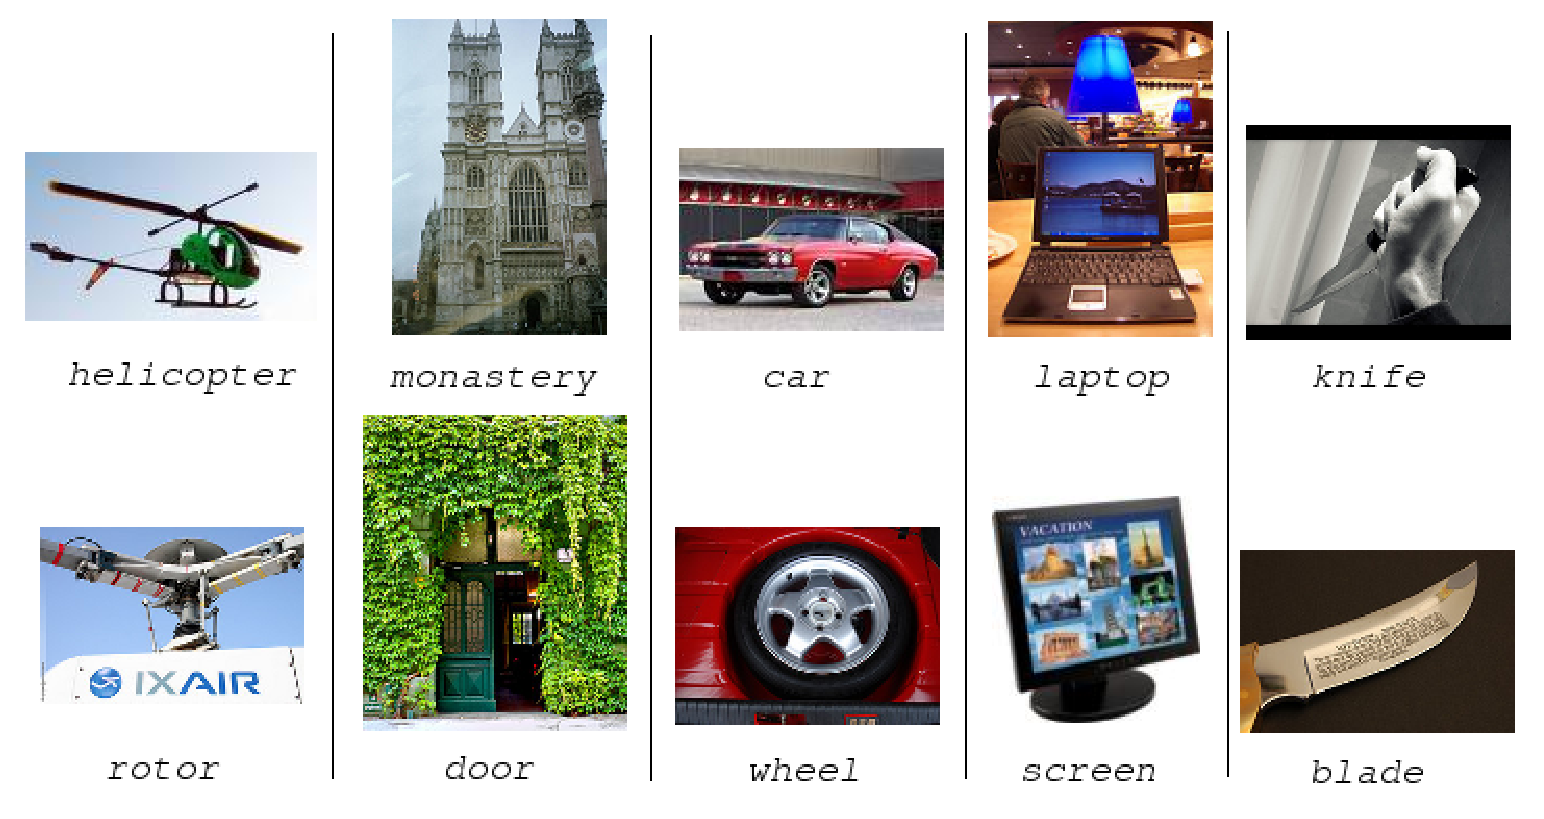
\includegraphics{article5/images/imnet3.eps} }

    \caption[Quadruplets from ImageNet+WordNet dataset]{{\bf Quadruplets from ImageNet+WordNet dataset} e.g ''rotor'' is
    \textit{part-of} ''helicopter''. Note that objects and their parts are not
    coming from the same image}

    \label{fig:quad}
    \end{center}
\end{figure*}

% Gregoire: 1) Repetition with section 4.1 2) maybe precise we are considering
% both cases Image/Word net where the part-of image is not taken from the same
% image and labelme where the part-of is actually from the same image. Think it
% would be better to wrote it in the LabelMe section



\subsubsection{Proxy Training Method}

% \paragraph{Proxy Data}
% We are given no direct supervision for our task of interest.
% We have two sources of data that we use: (1) a set of object labels and their semantic relation
% to each other (e.g. ``part-of'') which comes from WordNet; and (2) a set of images and their labels which
% comes from ImageNet.
% As a proxy to our task of interest we can hence build
% pseudo-positive examples that are quadruplets of the form $(I_o,L_o,I_p,L_p)$
% where $I_o$ and $L_o$ is an image and its label from ImageNet and $I_p$ and $L_p$ are also an image and label
% from ImageNet such that {\text{has\_part}}$(L_o,L_p)$ is a known relation in WordNet.

\paragraph{Proxy Ranking Task}

Given a positive quadruplet  $x = (I_o,L_o,I_p,L_p)$ we find the parameters that try to satisfy two kinds of 
constraint:
\begin{equation} \label{con1}  
   f_q(I_o,L_o,I_p,L_p) > f_q(I_o,L',I_p,L_p), ~~~ \forall L' \neq L_o
\end{equation} 
\begin{equation} \label{con2}  
   f_q(I_o,L_o,I_p,L_p) > f_q(I_o,L_o,I_p,L'), ~~~ \forall L' \neq L_p
\end{equation} 
In practice not all training data constraints can be satisfied so we instead optimize a {\em ranking loss}
that tries to optimize the precision at the top of the ranked list of labels.
%For constraints of the the first type, 
Following the loss defined in \citep{usunier,wsabie} 
we would like to minimize (for a single training example):
\[
   {\cal E} \left(rank_o(f_q(x))\right)  +    {\cal E} \left(rank_p(f_q(x))\right) 
\]
where:
\[
  rank_o(f_q(x)) =  \sum_{L' \neq L_o}  I( f_q(I_o,L',I_p,L_p) \geq f_q(x)),
\]
\[
  rank_p(f_q(x)) =  \sum_{L' \neq L_p}  I( f_q(I_o,L_o,I_p,L') \geq f_q(x)),
\]
i.e. $rank_o$ counts the number of labels that are ranked above the true object label 
and $rank_p$ counts the number of labels that are ranked above the true part label, and
\[
 {\cal E}(k)  =  \sum_{j=1}^k \alpha_j, \text{~with~} \alpha_1 \geq
 \alpha_2\geq \dots \geq 0
\]
is a function that transforms the ranks into a loss. 
If the first few indices of $\alpha$ index large values and smaller values follow this 
gives more weight to optimizing the top of the ranked list \citep{usunier}.
In our experiments we set  $\alpha_1=1$ and 
$\alpha_{j>1}=0$ to optimize the proportion of top-ranked correct labels.


\paragraph{Object and Part Training Algorithm}

Following the authors of \citep{wsabie} we optimize such a loss function via 
stochastic gradient descent by iterating over the following scheme:
\begin{enumerate}
\item Select a positive training quadruplet $x$ at random.
\item Select at random either constraint~\eqref{con1} or \eqref{con2}.
\item Set $N=0$.
\item Repeat:
{
  \begin{enumerate}
  \item Create a negative triplet $\tilde{x}$ by sampling a label $L'$ at random 
and constructing  $\tilde{x} = (I_o,L',I_p,L_p)$ for constraint~\eqref{con1}  
or $\tilde{x} = (I_o,L_o,I_p,L')$ for constraint~\eqref{con2}.
  \item N=N+1
  \end{enumerate}
}
until $f_q(x) > f_q(\tilde{x}) + 1$ or $N \geq \gamma$.
\item Make a stochastic gradient step to minimize
  ${\cal E}(\floor{\frac{\gamma}{N}}) |1-f_q(x)+f_q(\tilde{x})|_{+} $.
\item Enforce the constraints that each column $||W_i|| \leq 1$, $||V_i|| \leq 1$, $\forall i$ (this only involves updating the parameters that have changed in the gradient step).
\end{enumerate}

%For training we take a quadruplet (I_O,L_O,I_P,L_P)  as a positive example and create 2 negatives examples (I_O,RANDOM_LABEL_1,I_P,L_P) and (I_O,L_O,I_P,RANDOM_LABEL_2).
%(RANDOM_LABEL 1 and 2 are different)
%We perform forward-backward with these 2 pos-neg pairs. If there is no margin violation, we sample new negatives (WARP loss style).

Similarly to the method previously described in Section~\ref{warp}, 
step (4) approximates the calculation of
$rank_o$ or $rank_p$ rather than explicitly calculating them: instead of counting
all violating constraints one keeps sampling $N$ times (up to a maximum of $\gamma$) 
until one finds a single violating constraint.
The rank is then approximated with  $\frac{\gamma}{N}$ instead of using the true rank. 
Intuitively, if we have to sample for a long time to
find a violating constraint, the true rank must be relatively small.
This results in practically useful algorithms in terms of training time.

\paragraph{Hyperparameters}

We use an embedding dimension of $D=\{ 50,100 \}$ in all our experiments. For
sampling negative samples, we choose $\gamma\in\{10,100\}$ on various size of
mini-batch $\{100,1000\}$. The learning rates are set to $\{0.01,0.001\}$ for
$W,U$ and $\{0.1,0.01\}$ for $V$. 

For the image mapping $\Phi(\cdot)$ we use a
standard bag-of-visual-terms type representation, which has
a sparse vector representation. In particular, we use the bag-of-terms 
feature setup of \citep{grangier:2008:tpami}, which
was shown to perform well on image ranking tasks. 
The image is first segmented into several overlapping square blocks at various scales.
Each block is then represented by the concatenation of color and edge features.
These are discretized into a dictionary of $N = 10,000$ blocks,
by training k-means on a large corpus of images. Each image
can then be represented as a bag of visual words: a histogram
of the number of times each visual word was present in the
image, yielding $N$ dimensional vectors with an average of 245 non-zero values. 

\section{Related Work}\label{sec:rwork}

\paragraph{Part-based approaches}
There has been extensive work on decomposing objects into parts, and
using parts and their relations to model objects and their shapes.
Usually, the ``parts'' in these approaches are not viewed as isolated
objects by their own merits (like the flashlight of a camera), but
rather capture recurring patterns in patches that cover parts of the
images (like a bottom left side of a camera).
%
For example, \citep{agarwal2004learning} learned
models of parts and their spatial relations from sets of patches in
images, and then used them to label objects, such as cars in urban
environments. The current work has a different aim of explicitly
tagging the presence of parts in images. Another related work is by
\citep{crandall2006weakly}, who used a Markov random field to learn a
rich appearance and shape model with training data that only had class
labels. Once again the parts learned in this work do not correspond to
smaller objects but rather to patches that cover parts of objects.

\paragraph{Object Detection using Part or Attribute-based models}

Using parts or attributes has shown promising results for object detection.
\citep{core} build an object representation where objects are described as a
collection of semantically meaningful attributes e.g. parts, material.  Also, \citep{fel2009}
shows how to train state of the art object detectors which first localize
parts of an object in combination with a whole object detector.
These approaches differ from ours since we are focusing
on classification and image retrieval and not on detection.



\paragraph{Image labeling with embedding-based models}

The idea of using embedding algorithms for image labeling has been tried
using several varying methods.
PLSA \citep{monay2004plsa} was applied but has been shown to perform
worse than (non-embedding based) supervised ranking models such as the large margin classifier
 {\sc Pamir} \citep{grangier:2008:tpami}. Embedding for image retrieval (rather than annotation)
using KCCA was also explored in \citep{zhou2007semi}.
The most related work to ours is that of \citep{wsabie} which uses a ranking criterion
optimizing the top of the ranked list like ours to label images where they obtained very good
results compared to non-embedding approaches (such as {\sc Pamir}) on large scale tasks.
None of these works however explored labeling parts in images.
The current work aims to learn richer models which incorporate both
 image-label similarity functions and object-label to part-of-label similarity functions.
We focus on the difficulty of training such models 
%utilize multitasking with relations  
%in WordNet to deal with 
given a lack of large-scale supervision for the part-based tasks we are interested in.


\section{Empirical Evaluation}\label{sec:exp}


We first briefly give experimental results in an image annotation setup which
labels {\em objects only} (Section~\ref{sec:oos}).  These results justify the
general embedding approach and choice of loss function that we use in the rest
of our experiments on objects and parts, and are a summary of the results from
\citep{image-wsabie}.  Then, we present new results for the object and part
model we are interested in (Sec.\ref{sec:ops}).

\subsection{Objects Only}\label{sec:oos}

The approach we advocate in this setup is to use the embedding
algorithm detailed in Section \ref{jwie} with the WARP loss of Section
\ref{warp}.  This method is called {\sc WSABIE} (Web Scale Annotation
By Image Embedding).




\paragraph{Dataset}

ImageNet~\citep{imagenet_cvpr09}
is a large-scale image dataset organized according to WordNet~\citep{wordnet:1998}.
Concepts in WordNet, described by multiple words or word phrases, are
hierarchically organized. ImageNet is a growing image dataset that attaches
quality-controlled human-verified images to  these concepts.
The version that was downloaded for these experiments had 
4.1 million images and 15,952 classes.
The data was split into 2.5M images for training, 0.8M for validation and
0.8M for testing, removing duplicates between train, validation and test
by throwing away test examples which had too close a nearest neighbor training
or validation example in feature space.

\paragraph{Feature Representations}

As mentioned before, we will consider a bag-of-visual-terms type representation,
but many other types of feature representation appear in the literature.
We hence also explored the possibility that an ensemble of feature representations that can 
improve performance as has been shown before \citep{makadia:2008}.
We thus combined multiple feature representations which are the
 concatenation of various spatial \citep{pyramid} and multiscale color and
texton histograms \citep{textons}
for a total of about $5 \times 10^5$ dimensions.
% The descriptors are
%somewhat sparse, with about 50000 non-zero weights per
%image. Some of the constituent histograms are normalized
%and some are not.
We then perform Kernel PCA \citep{kpca} on the combined feature representation using the intersection
kernel \citep{intersection-kernel} 
to produce a 1024 dimensional input vector for training {\sc Wsabie}. We then train {\sc Wsabie} as before.


\begin{table}[t]
\caption[Test Set Results on ImageNet]{\label{table:imagenet-perf} {\bf Summary of Image Annotation (Object labeling only) Test Set Results on ImageNet.} Precision at 1 and 10 are given.}
\centering
\begin{small}
\begin{tabular}{|l||c|c|c|}
\hline
Algorithm         & Features used       & p@1     & p@10  \\
\hline
{Approx.} {\sc $k$-NN}     & Bag of Visterms          & ~1.55\%~~  & - \\
{Exact} {\sc $k$-NN}       & Bag of Visterms          & ~4.50\%~~  &  - \\
{One-vs-Rest} Linear Machine    & Bag of Visterms             & ~2.27\%~~  & 1.02\% \\
AUC Ranking-loss Linear Machine  & Bag of Visterms             & ~3.14\%~~  & 1.26\% \\
{\sc Wsabie} [d=500]           & Bag of Visterms             & ~6.14\%~~  & 2.09\% \\
\hline
Exact $k$-NN               & Ensemble+KPCA        & ~7.73\%  &   -   \\
{\sc Wsabie} [d=1000]      & Ensemble+KPCA             & 10.03\% & 3.02\% \\
\hline
\end{tabular}
\end{small}
%o\vskip -0.1in
%\end{table}
%\begin{table}
\caption[WARP versus AUC optimization]{\label{table:imagenet-owpc} {\bf  WARP vs. AUC optimization.} 
We compared the two types of loss function WARP and AUC or two types of model:
semantic embedding models and linear models.
For both model types, WARP improves over AUC.
\label{fig:warp-vs-auc}
}
\centering
\begin{small}
\begin{tabular}{|l|l|c|c|}
\hline
 Model &  AUC ~~p@1~~  & WARP ~~p@1~~ \\
\hline
% {{\bf Dataset:} ImageNet} & & &  \\
 $f(I_o, L_o) = (V \Phi_I(I_o))^\top W_{\Phi_L(L_o)}$~~[D=100]   & 1.65\%  & {\bf4.03\%}  \\
 $f(I_o, L_o) = w_i^\top  \Phi_I(I_o))$  & 3.14\%  & {\bf 4.25\%}  \\
\hline
\end{tabular}
\end{small}
\end{table}






\paragraph{Baselines}

We compare the embedding approach WSABIE
to several baselines: 
approximate $k$-nearest neighbors ($k$-NN),  exact $k$-NN
one-versus-rest linear large margin classifiers (One-Vs-Rest) of the form 
$f(I_o, L_o) = w_i^\top  \Phi_{\cal I}(I_o)$ trained separately for each class $L_o$,
or the same models trained with an AUC type ranking loss instead (sometimes called the multiclass loss).
For all methods, hyperparameters are chosen via the validation set.

%While One-vs-Rest  and \Multiclass have the same form, the latter is 
%trained with a margin ranking loss which couples the classifiers,
%rather than independently training
%binary classification loss. Note however that One-Vs-Rest can easily be
%trained in parallel while \Multiclass cannot.

We tested approximate $k$-NN because $k$-NN is often not feasible. There are many
flavors of approximation (see, e.g \citep{Fergus:small_codes}). We chose the following: 
a random projection at each node of the tree is chosen
with a threshold to go left or right that is the median of the projected training data to make the tree 
balanced. After traversing $p$ nodes we arrive at a leaf node containing
$ t \approx n/2^p  $ of the original $n$ training points from which we calculate the nearest neighbors. 
Choosing $p$ trades off accuracy with speed.

\paragraph{Metrics}

We compared our models using the precision at the top k of the list
(p@k). This metric gives more
importance to the true annotations appearing in the top of the list and is defined as:

\[
  \textrm{p@k} = \frac{1}{N} \sum_{i=1}^{N} \dfrac{I\{\textrm{PredictedRank}(x_i)< k\}}{k}
\]

where $N$ is the size of the set, $x_i$ is an image and its label, PredictedRank
a function that returns the rank of $x_i$ according to the considered
score function and $I\{X\}$ returns the number of elements of the set $X$.

\paragraph{Results}

The results of  comparing all methods on ImageNet are summarized in Table \ref{table:imagenet-perf}.
As expected, the choice of feature representation has a large impact on the results. The ensemble+KPCA features
outperform Bag of Visterms independent of the learning algorithm. However, for both feature types
{\sc Wsabie} outperforms the competing methods tried. The choice of embedding dimension 
$D$ for {\sc Wsabie} is given in the Table. Smaller values give slightly worse results, 
e.g. $D=100$ with Bag of Visterms gives $4.03\%$.


We also compared  different models trained with either WARP or AUC
 optimization: either the embedding approach of {\sc Wsabie} ($D=100$) or a full linear model.
The results given in Table \ref{fig:warp-vs-auc} show WARP 
gives superior performance.




\subsection{Objects and Parts} \label{sec:ops}

In this Section we present results with our models that learn the semantics of
both objects and their parts.

\begin{table}[t!]
\begin{center}
\caption[Results on ImageNet-WordNet]{\textbf{Summary of Test Set Results on ImageNet-WordNet.}
Precision at 1 and 10, and Mean Reciprocal Rank (MRR) are given.
(IW) resp. (I) refers to the (Image,Word) setup resp. (Image).\label{tab:iw}}
\resizebox{1\linewidth}{!}{
\begin{tabular}{|l||l|l|l||l|l|l||l|l|l|} %{|l|p{8cm}|}
\hline
& \multicolumn{3}{c||}{Image Annotation} & \multicolumn{3}{c||}{Part-Object Labeling} &  \multicolumn{3}{c|}{Triplet}\\
Models & p@1 & p@10 & MRR & p@1 & p@10 & MRR & p@1 &p@10 & MRR\\
\hline
Shared (IW)     & --            & --          & --          & \textbf{11.48\%} & \textbf{3.40\%} &\textbf{0.1892} & 26.31\% &\textbf{9.90\%} & 0.5545 \\
UnShared (IW)   & --            & --          & --          & 10.01\%        & 3.02\% & 0.1669 & \textbf{33.13\%} & 9.62\% & \textbf{0.5595} \\
\hline
Shared (I)      &  11.21\%          & 3.85\%          & 0.2021          & 5.13\%  & 1.84 \% & 0.0955 &  11.21\%          & 3.85\%          & 0.2021  \\
UnShared (I)    &  \textbf{12.94\%} & \textbf{4.10\%} & \textbf{0.2219} & 6.08\% &  2.11\%  & 0.1118 &  12.94\% & 4.10\% & 0.2219\\
\hline
SVM & 10.02\% & 3.72\% &  0.1864 & -- & -- & -- & 10.02\% & 3.72\% &  0.1864 \\
\hline
\end{tabular}
}
\end{center}
\end{table}



\subsubsection*{Notation summary}

\begin{itemize}

\item $f_{IW}^S : {\cal I} \times {\cal L} \times {\cal I} \times {\cal L}
\rightarrow {\mathbb R}$ returns a score given a quadruplet of images and
annotations of a part and an object. This model uses the same semantic space
for encoding the WordNet relationships and image visual similarities.

\item $f_{IW}^U : {\cal I} \times {\cal L} \times {\cal I} \times {\cal L}
\rightarrow {\mathbb R}$  uses different unshared semantic spaces for
WordNet relationships and image visual similarities.
 

\item $f_{I}^S : {\cal I} \times {\cal L} \times {\cal I} \times {\cal L}
\rightarrow {\mathbb R}$  shares the same semantic space for part-of
relationships and image visual similarities but does not use the Part-Object score
$f_{L}$ for ranking.

\item $f_{I}^U : {\cal I} \times {\cal L} \times {\cal I} \times {\cal L}
\rightarrow {\mathbb R}$ corresponds to the original WSABIE system.

\end{itemize}



\paragraph{Models}

We consider two models denoted ``Shared'' and ``Unshared''. The
``Shared'' model shares the label embedding matrix $W$ for both
functions $f_I$ and $f_L$, and the ``Unshared'' model has an
additional label embedding matrix $U$ for $f_I^U$ (see
Section~\ref{sec:jmodels}). 

The two models are considered in two different setups.  In the first
case, ``Image-Word'', the score of a quadruplet $(I_o,L_o,I_p,L_p)$ is
computed using images and word label-label interactions. The score
function for the ``Shared'' model is:

\[
f_{IW}^S(I_o,L_o,I_p,L_p) = f_I(I_o,L_o) + f_I(I_p,L_p) + \alpha f_{L}(L_o,L_p) 
\]

and for the ``Unshared'' model:

\[
f_{IW}^U(I_o,L_o,I_p,L_p) = f_I^U(I_o,L_o) + f_I^U(I_p,L_p) + \alpha f_{L}(L_o,L_p)
\]


where $\alpha$ is an hyperparameter set to $0.1$ in our experiments.


In the second case (denoted ``Image''), the score is given by image-label interactions only
(it does not use the within-labels score $f_L$) in the ``Shared'' model:

\[
f_I^S(I_o,L_o,I_p,L_p) = f_I(I_o,L_o) + f_I(I_p,L_p) .
\]

and in the ``Unshared'' model:

\[
f_I^U(I_o,L_o,I_p,L_p) = f_I^U(I_o,L_o) + f_I^U(I_p,L_p) .
\]

As a baseline classifier, we also compare our models with a multiclass SVM
trained in a one-vs-rest setting with LibLinear~\citep{liblinear}.



%on a subset of $100$k training couples (Image,Label) instead of
%$324$k.

\paragraph{Metrics}

As before, we compared our models using the precision at the top k of the list
(p@k), as well as the mean reciprocal rank (MRR), which is defined as:
\[
  \textrm{MRR} = \frac{1}{N} \sum_{i=1}^{N} \dfrac{1}{\textrm{PredictedRank}(x_i)},
\]
where $N$ is the size of the set, $x_i$ is a quadruplet, PredictedRank
a function that returns the rank of $x_i$ according to the considered
score function and $I\{X\}$ returns the number of elements of the set $X$.

\paragraph{Tasks}%{Standard Image Annotation} % task 1.
We consider three different tasks.

The first task, termed {\bf Image Annotation}, is a standard image labeling
task where our part-based architecture is not really useful, but still serves
as a kind of sanity check of our system. Given one image $I_o$ of an object or
a part $I_p$, the model has to predict the correct label among $K=1000$
different synsets.
%
This task is used to assess the basic quality of our image labeling model
$f_I^U$ or $f_I^S$ w.r.t. the SVM.  Since the Image-Word models use $f_L(.,.)$
to compute the ranking score which has no relation whatsoever with the image
property, we will not evaluate them in this task.

% \[
%     \argmax_{L'_o}  f_O(I_o,L'_o) \textrm{ and } \argmax_{L'_p} f_P(I_p,L'_p).
% \]

%\paragraph{Joint Part-Object Labeling} % task 2.

Our second task, termed {\bf Part-Object Labeling}, is particularly of
interest for our setting to evaluate the gain of using a joint
prediction model using image and words as we propose.  Given an object
$I_o$ and a part $I_p$, one has to predict the correct pair of
labels $(L_o,L_p)$ over $K^2=1$M possible pairs.

% \[
%     \argmax_{L'_o,L'_p}  f(I_o,L'_o,I_p,L'_p).
% \]

%\paragraph{Label Prediction given a Triplet} % task 3

Our third task, termed {\bf Triplet}, is derived from the previous, but it assumes that
either the object $I_o$ or the object part $I_p$ has already been
labeled (or is known using prior knowledge).  Hence, given a pair of
images $I_p$ and $I_o$, and the label of either the part $L_p$ or the
object $L_o$, the model has to correctly predict the missing label.

% \[
%     \argmax_{L'_p}  f(I_o,L_o,I_p,L'_p) \textrm{ or }  \argmax_{L'_o}  f(I_o,L'_o,I_p,L_p).
% \]

The two last tasks use the ranking functions $f$ as defined above i.e $f_{IW}^U$,
$f_{IW}^S$, $f_I^U$ and  $f_I^S$ depending on the setup of the models that are
being evaluated.  The best models are selected w.r.t. their mean rank error on
the joint part-object labeling task by using $f_{IW}^S$, $f_{IW}^U$, $f_I^S$ or
$f_I^U$ computed on $50$k quadruplets of the validation set from
ImageNet+WordNet and ranked over $1$ M  pairs. 

\paragraph{Training and Testing}


The difference between the Shared (Image) and Unshared (Image) appears during
training. Considering {\bf Image Annotation}, even if $f_L$ is not used for
computing the score at the end, the training process will perform a gradient
step on $W$ with respect to $(L_p,L_o)$, $(I_o, L_o)$ and $(I_p,L_p)$ for the
shared model while the unshared parameters only receive updates coming from
$(I_o,L_o)$ and $(I_p,L_p)$.

Unshared (Image) is similar to the original WSABIE model
and is presumably better than Shared (Image) which will push part-object word
embeddings to be closer. For example in the Shared (Image) model, {\it car} and
{\it wheel} will be close in the embedding space but having {\it wheel} ranked high
for {\it car} is naturally not optimal.






\subsection{ImageNet-WordNet Data}

Results on the test set of our custom data are presented in Table~\ref{tab:iw}.
%
On the standard {\bf Image annotation} task, all considered models reach
reasonable performance and compare nicely with the SVM.  We would expect that
the models using (I)
%and those using (IW)
would achieve the same value because on this particular task.
%, the $f_L$ score that differentiates them is not used.
However our models are selected using a validation score on the {\bf
Part-Object Labeling} and thus different configurations are picked, resulting
in different performances.




On the {\bf Triplet} task, models (I) have the same performance as for 
{Image annotation} because they are unable, by construction, to use the information
coming from the already assigned label. Models (IW) using that
information experience an increase in accuracy for all criteria: using
the within-label score $f_L$ is a major plus that these methods can
exploit. They reach values of  33.13\% p@1 which on a
task with 1,000 labels is a fairly remarkable achievement.

Results of the {\bf Part-Object Labeling} task
confirm the usefulness of using our joint scoring model. Indeed, both
models (IW) using all scores clearly outperform the competing methods. 
On top of that, sharing embeddings during training brings an additional
improvement because the labels have acquired richer representations
through their multi-task training within $f_I$ and $f_L$.


%%%%% 
\subsection{LHI Data}
We further evaluated our models on a set of objects pairs that were
manually annotated as objects and their parts. To create this data, we
used a set of images annotated by Labelme \citep{labelme} and parsed
by the Lotus Hill Research Institute (LHI)~\citep{yao2009image}. 

\paragraph{Data collection}
We downloaded the LHI data from {\em yoshi.cs.ucla.edu/yao.data/}. For
every image, this dataset contains an annotation of the image and list
of bounding boxes surrounding parts of the object together with the
annotation of all parts. We manually matched these annotations with
the list of WordNet synsets (for example by matching the term 'camera'
to the relevant synset ``n03358726''). We then intersected the list of
synset-pairs which exist in ImageNet with the list of annotation pairs
in the LHI data, and extracted images of parts from the bounding
boxes. This yielded a set of image pairs, each having an object and
its part, and each labeled with a synset that can be modeled using
ImageNet. An example of such a set is depicted in Figure~\ref{fig:labelme}.


The LHI data contains $489$ image pairs (Object,Part) with $19$ \textit{part-of}
relations. Note that $10$ of those relations do not appear in our training set.
%These real-world conditions made this task particularly challenging. 
A perfect example: ''Propeller is \textit{part-of} Wing is \textit{part-of} Aircraft''.
''Propeller is \textit{part-of} Aircraft'' is not in our training set of $771$
relations but ''Propeller is \textit{part-of} Wing'' and ''Wing is
\textit{part-of} Aircraft'' are.
%
Moreover, it is also important to add that the patches representing
objects are also usually in a much lower resolution than the images from
ImageNet.

\begin{figure*}[t!]
  \begin{center}
    \resizebox{0.8\textwidth}{!}{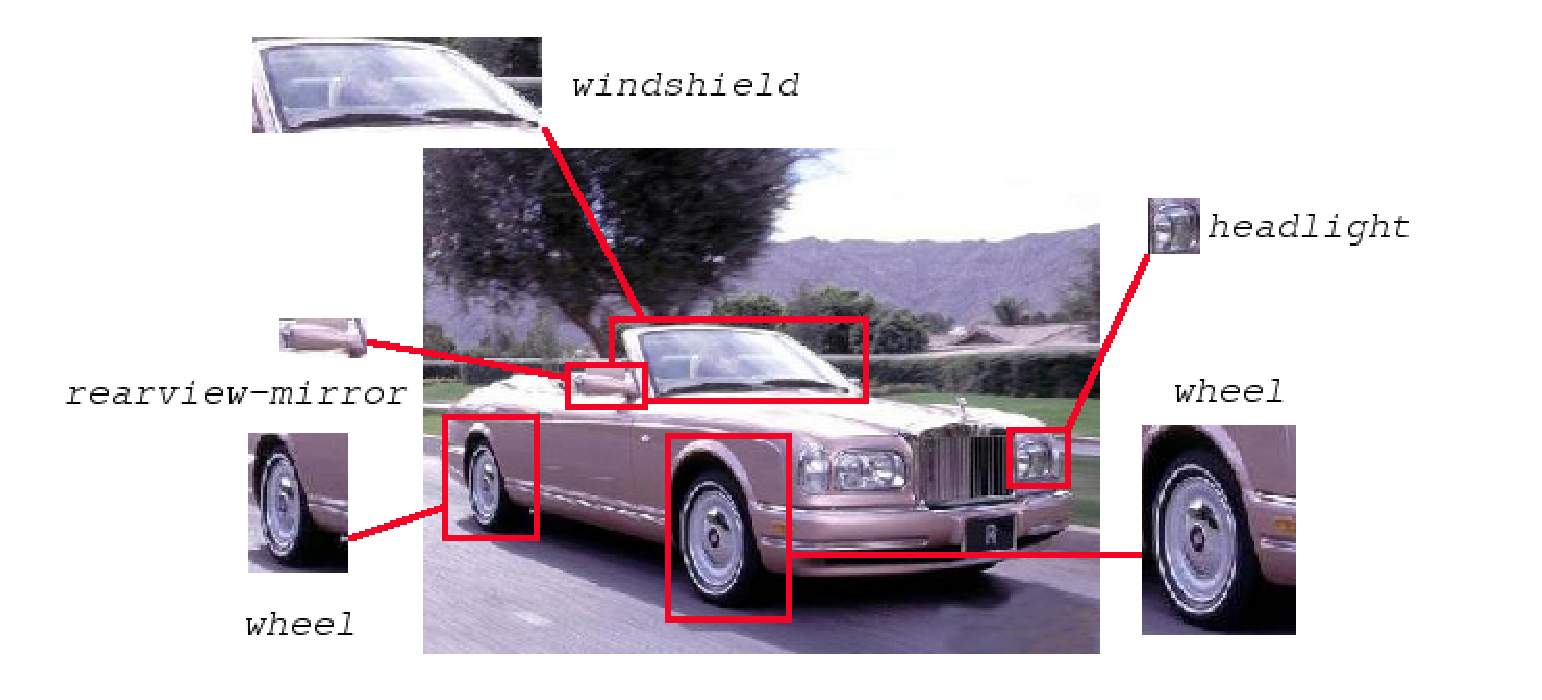
\includegraphics{article5/images/labelme.eps} }
    \caption[Example from LHI data]{{\bf Example from LHI data} depicting an image of an object and its parts.}
    \label{fig:labelme}
    \end{center}
\end{figure*}



\paragraph{Results} This evaluation set is harder than the previous
one due to its real-world conditions. This is reflected in the results
presented in Table~\ref{tab:lhi}.
%
We can still draw the same conclusions as for the previous section.
That is, using the within-label score improves performances i.e. (IW)
is always better than (I).
%
Furthermore, these results show that our proxy supervision is
useful and allows the model to learn a prediction function that
can nicely transfer to real-world data even though such data {\it has
  never been seen in training}.
%




\begin{table}[t!]
\begin{center}
\caption[Results on LHI data]{\textbf{Summary of Results on LHI data}\label{tab:lhi}}
\resizebox{1\linewidth}{!}{
\begin{tabular}{|l||l|l|l||l|l|l||l|l|l|} %{|l|p{8cm}|}
\hline
& \multicolumn{3}{c||}{Image Annotation} & \multicolumn{3}{c||}{Part-Object Labeling} &  \multicolumn{3}{c|}{Triplet}\\
Models & p@1 & p@10 & MRR & p@1 & p@10 & MRR & p@1 &p@10 & MRR\\
\hline
Shared (IW)     & --  & --   & --  & \textbf{0.25\%}   &\textbf{0.13\%} &\textbf{0.0075}  & 9.10\%  & 4.43\%   &  0.2044    \\
UnShared (IW)   & --  & --   & --  & 0.0\%  & 0.10\%  & 0.0043   &\textbf{18.20\%}  &\textbf{4.79\%}  &\textbf{0.2778}  \\
\hline
Shared (I)      & \textbf{10.85\%}  &\textbf{2.92\%}  &\textbf{0.1728}  & 0.0\%  & 0.08\%   & 0.0039  & 10.85\%  & 2.92\%  &0.1728 \\
UnShared (I)    & 7.26\%  & 2.37\%  & 0.1288  & 0.0\%  & 0.03\%   & 0.0025  & 7.26\%  & 2.37\%  & 0.1288  \\
\hline
\end{tabular}
}
\end{center}
\end{table}

\subsection{WordNet tree and generalization to unseen relationships}

The Image-Word models (Shared and Unshared) learn an embedding encoding the
part-of relationships but one can think of directly using the WordNet tree.


\subsubsection*{Notation summary}

\begin{itemize}

\item $f_{IO}^S : {\cal I} \times {\cal L} \times {\cal I} \times {\cal L}
\rightarrow {\mathbb R}$  shares the same semantic space for part-of
relationships and images visual similarities. An offset is added to the ranking
score if the part-of relationship was present in the training set.

\item $f_{IO}^U : {\cal I} \times {\cal L} \times {\cal I} \times {\cal L}
\rightarrow {\mathbb R}$ corresponds to the original WSABIE system where an
offset is added to the score in the same way as before in order to filter out
the training relationships.

\end{itemize}


 In order to use this prior in the Image models (Shared and Unshared), we add
 an offset to the original score if the part-of relationship is in the training
 set:


\[
f_{IO}^S(I_o,L_o,I_p,L_p) = f_{I}^S(I_o,L_o,I_p,L_p) + O(L_p,L_o).
\]

\[
f_{IO}^U(I_o,L_o,I_p,L_p) = f_{I}^U(I_o,L_o,I_p,L_p) + O(L_p,L_o).
\]

where 

\[
O(L_p,L_o)=
\left\{
\begin{array}{rl}
\lambda & \textrm{if $(L_p,L_o)$ is in the training relationships.} \\
0 & \textrm{otherwise.}
\end{array}
\right.
\]

In addition,
% to highlight the performance of using the WordNet directly, 
we wanted to stress the ability of Image-Word models for generalizing to
unseen part-of relationships. Indeed given 'wheel is-part-of car' and that 'car'
shares visual similarities with 'truck', Image-Word models learn to push
truck-wheel embeddings together even if 'wheel is-part-of truck' is not present
in the training data.

The LHI dataset is particularly appropriate for these two experiments. All the models
have been trained on $771$ part-of relationships but $50\%$ of the part-of
relationships in LHI ($10/19$) are not in those training relationships.  When
testing on the LHI dataset, we filtered out the results keeping all the part-of
relationships among these 781 couples ($771$ training relationships and $10$
unseen during training coming from LHI). Therefore, in the Image models score (Shared and
Unshared), an offset (we used $\lambda=100$ in our experiments) was added if the part-of
relationship was among the $771$ training relationships. The Image-Word models
(Shared and Unshared) are kept as before.

\begin{table}[t!]
\begin{center}

\caption[WordNet Tree and Unseen relationships]{\textbf{WordNet Tree and Unseen relationships}\label{tab:generalize}
Image-Word Shared models allow to generalize to unseen relationships. Using the
WordNet tree also improves the performance. (IO) refers to the original Image
where an offset was added to filter out relations both in the
WordNet tree and the training set. Part-Object relationships are ranked among $781$ couples.}

\resizebox{0.5\linewidth}{!}{
\begin{tabular}{|l||c|c|c|} %{|l|p{8cm}|}
\hline
&  \multicolumn{3}{c|}{Part-Object Labeling using WordNet}  \\
Models & p@1 & p@10 & MRR   \\
\hline
Shared (IW)     & \textbf{3.06\%}  & \textbf{2.45\%}   & \textbf{0.1005} \\ 
UnShared (IW)   & 2.04\%  & 1.64\%  & 0.0670  \\
\hline
Shared (IO)     & 1.43\%  & 1.17\%  & 0.0483  \\
UnShared (IO)   & 1.23\%  & 1.45\%  & 0.0519  \\
\hline
\end{tabular}
}
\end{center}
\end{table}


Results in Table~\ref{tab:generalize} highlight the advantage of using
Image-Word models, those are able to generalize to unknown relationships ($10$
relationships in LHI out of the training set) through word smoothing in the
embedding space.  Using the WordNet tree to filter out relationships among the
1M possible couples (by keeping only $781$ relationships) is also helpful as
the performance increased drastically for all models (in comparison with
results w/o using WordNet tree in Table~\ref{tab:lhi}).

\subsection{Encoded Semantics}

\begin{table}
\begin{center}
\caption[Nearest Neighbors of Word Embeddings]{\label{tab:embed}\textbf{Nearest Neighbors of word embeddings learned with Shared and Unshared models.}{\small Shared embeddings
 exhibit visual similarities in addition to semantics {\it e.g.} strings of an instrument and laces of a shoe, a radio-phonograph is usually set up on a desk or a dresser.}}
\resizebox{1\linewidth}{!}{
\begin{tabular}{|c|c||c|c||c|c|} %{|l|p{8cm}|}
\hline
\multicolumn{2}{|c||}{\bf Toe} & \multicolumn{2}{c||}{\bf Radio-phonograph} &  \multicolumn{2}{c|}{\bf Loudspeaker}\\
{\it shared} & {\it unshared} & {\it shared} & {\it unshared} & {\it shared} & {\it unshared}\\
\hline
footwear            & shoe              & dresser                & tuner&
 lens & public address system \\
tongue              & accelerator pedal & rotor head            & amplifier&
             sustaining pedal & amplifier \\
stringed instrument & storage           & firebox               & public address system &
  public address system & tuner\\
shoe                & boot              & rear light            & loudspeaker&
      optical instrument & radio-phonograph\\
\hline
%soundboard          & afterburner       & electric_typewriter   &
\end{tabular}
}
\end{center}
\end{table}


Example word embeddings learned by our shared and unshared models on the ImageNet-WordNet data
are given in Table~\ref{tab:embed}. We observe that the embeddings capture the semantic structure of the 
labels. Besides, the shared model also encodes some information regarding the visual aspect of the object (or part) in its features.
Hence, stringed instruments and shoes have strings and laces as parts, which are visually alike.

\begin{figure*}
  \begin{center}
    \resizebox{1.05\textwidth}{!}{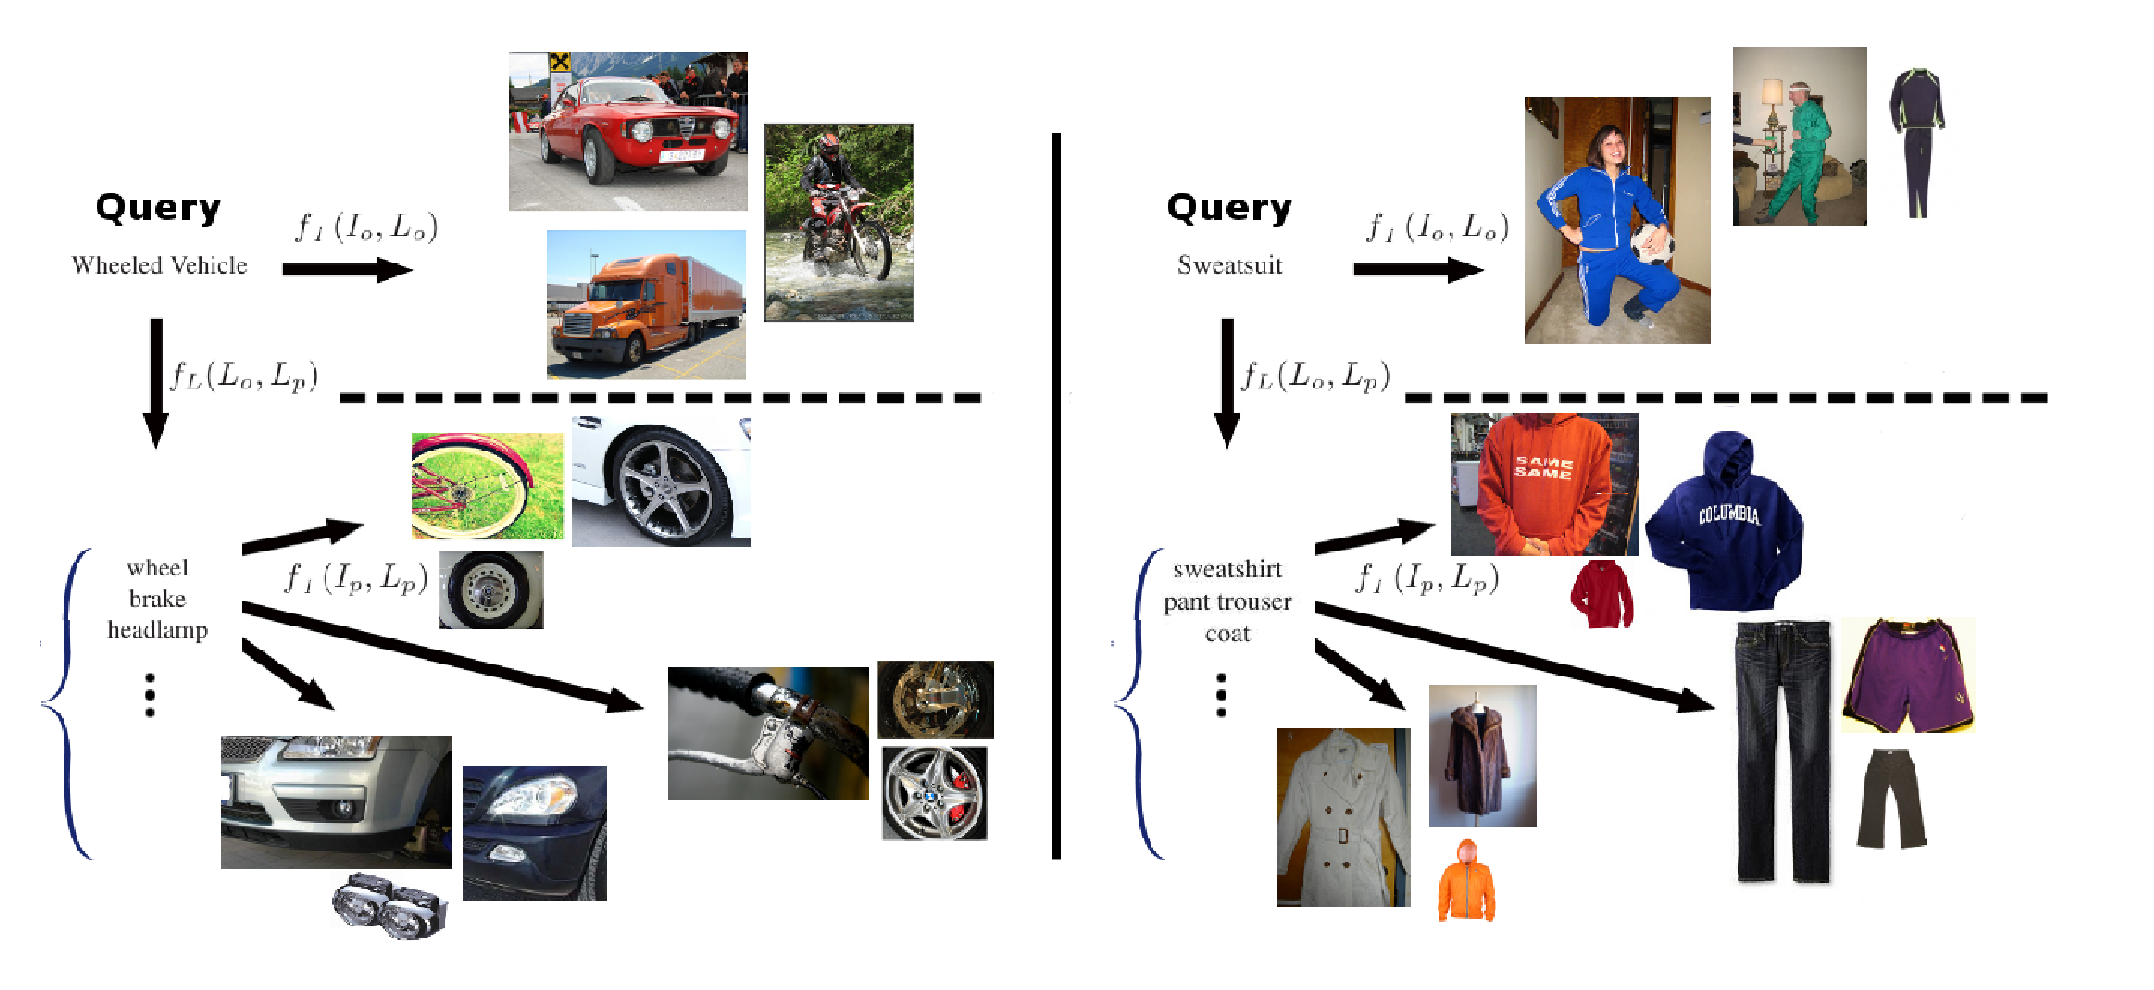
\includegraphics{article5/images/augmented3.eps} }
    \caption[Semantically Augmented Image Search]{\label{fig:sem_search}{\bf Semantically Augmented Image Search.} {\small For a given query 
    ("wheeled vehicule" on the left and "Sweatsuit" on the right), our model can retrieve corresponding images
    using $f_{I}$ (above the dashed line) but can also automatically extend the query to associated terms 
    (object parts in this work) using $f_{L}$ and hence retrieve semantically related images using $f_{I}$ 
    (below the dashed line). These results were obtained with the unshared model.}}
    \end{center}
\end{figure*}


Figure~\ref{fig:sem_search} illustrates an application for which our model could readily be applied, which 
we could term {\it semantically augmented search}. Given a text query, our model can retrieve corresponding 
images using the $f_I$ function, as standard {\it object only} image retrieval approaches do.
However, for no additional cost, 
our model can also extend the original query by searching for semantically associated terms (which are only parts in our current work) 
using the $f_L$ function, and can finally return part images related to those by leveraging the $f_I$ function.
%
Therefore, our model can generalize an image query to search for other objects which have little 
or no visual similarity with the original object of interest but are semantically linked to it, hence improving the original search and browsing experience.
%
This is related to recent efforts on attribute-based search pulled off by search engines.

\section{Conclusion and Future Directions} \label{conclusion}

This paper presented an original approach to learn to automatically 
tag images with their objects and their object-parts.
%
In particular, we proposed a proxy supervision that allows to
bypass the high cost of annotating such data.
%
We illustrated this setting by introducing a new dataset created by
connecting  ImageNet and WordNet through part-based within-label
relations.
%
We also presented a model that can be trained under such an indirect
supervision by jointly encoding both object image to object label, and
object label to object part label similarities.
%
Our experimental evaluation performed on our custom test set as well
as on exhaustively annotated data showed that this model can be
successfully trained under our proxy supervision.

Our idea of merging vision and semantic data is not limited to
labeling objects and object parts.
%
We chose this setting because it may be the most obvious and
because it has many potential applications.
%
However, our proxy supervision and our associated algorithm could also
be used in other contexts and with other databases.
%  For example, by keeping ImageNet and
% WordNet, one could leverage the information of the {\it hypernym}
% relations (i.e. {\it type-of}) of WordNet. By doing so one could train
% a model to label objects in images with 
%
For instance, one could think of connecting Labeled Faces in the
Wild (LFW)~\citep{LFWTech} as the image data and Freebase~\citep{freebase} as
the semantic graph among labels.
%
Indeed, Freebase proposes a vast graph linking persons with various
relations such as {\it married-to}, {\it son-of}, etc. that matches
well the set of labels of LFW.
%
By connecting these two resources, one could build up a model able to
leverage some underlying connection between the members of a group picture
to jointly label them. 
%
This is just an example of future directions/applications that could
be explored with our new proxy supervision for image annotation.

\section{Acknowledgements}

This work was supported by the DARPA Deep Learning Program, NSERC, CIFAR, the
Canada Research Chairs, Compute Canada and by the French ANR Project ASAP
ANR-09-EMER-001. Codes for the experiments has been implemented using both
Torch \citep{collobert:2011c} and Theano \citep{bergstra+al:2010-scipy} Machine
Learning libraries.




%{\small
%\bibliography{myrefs,biblio}
%\bibliographystyle{plain}
%}



\if 0
\section{Introduction}
\label{intro}
Your text comes here. Separate text sections with
\section{Section title}
\label{sec:1}
Text with citations \citep{RefB} and \citep{RefJ}.
\subsection{Subsection title}
\label{sec:2}
as required. Don't forget to give each section
and subsection a unique label (see Sect.~\ref{sec:1}).
\paragraph{Paragraph headings} Use paragraph headings as needed.
\begin{equation}
a^2+b^2=c^2
\end{equation}

% For one-column wide figures use
\begin{figure}
% Use the relevant command to insert your figure file.
% For example, with the graphicx package use
%  \includegraphics{example.eps}
% figure caption is below the figure
\caption{Please write your figure caption here}
\label{fig:1}       % Give a unique label
\end{figure}
%
% For two-column wide figures use
\begin{figure*}
% Use the relevant command to insert your figure file.
% For example, with the graphicx package use
%  \includegraphics[width=0.75\textwidth]{example.eps}
% figure caption is below the figure
\caption{Please write your figure caption here}
\label{fig:2}       % Give a unique label
\end{figure*}
%
% For tables use
\begin{table}
% table caption is above the table
\caption{Please write your table caption here}
\label{tab:1}       % Give a unique label
% For LaTeX tables use
\begin{tabular}{lll}
\hline\noalign{\smallskip}
first & second & third  \\
\noalign{\smallskip}\hline\noalign{\smallskip}
number & number & number \\
number & number & number \\
\noalign{\smallskip}\hline
\end{tabular}
\end{table}


%\begin{acknowledgements}
%If you'd like to thank anyone, place your comments here
%and remove the percent signs.
%\end{acknowledgements}

% BibTeX users please use one of
%\bibliographystyle{spbasic}      % basic style, author-year citations
%\bibliographystyle{spmpsci}      % mathematics and physical sciences
%\bibliographystyle{spphys}       % APS-like style for physics
%\bibliography{}   % name your BibTeX data base

% Non-BibTeX users please use
\begin{thebibliography}{}
%
% and use \bibitem to create references. Consult the Instructions
% for authors for reference list style.
%
\bibitem{RefJ}
% Format for Journal Reference
Author, Article title, Journal, Volume, page numbers (year)
% Format for books
\bibitem{RefB}
Author, Book title, page numbers. Publisher, place (year)
% etc
\end{thebibliography}
\end{document}
\fi

% end of file template.tex

